\section{Przedstawienie wyników oraz omówienie}
Powyższe algorytmy miały na celu jak najdokładniej odwzorować obiekt na podstawie danych z kamery głębi. W poniższej sekcji omówione zostaną wyniki użytych metod. Ukazane zostaną modele utworzone poprzez wykorzystanie algorytmu BPA oraz triangulacji Delaunay'a. Przedstawiona zostanie dokładność odwzorowania powierzchni oraz procentowa zawartość dziur. W celu testów wykonano dwa skany przedmiotów. Dokonano przekształcenia na model 3D jabłka oraz pudełka. Oba te przedmioty mają swoje barwy które również zostały oddane w modelach.
\subsection{Algorytm BPA}
Dla algorytmu toczącej się kuli dokonano pomiaru wpływu promienia na ostateczny wygląd modelu. Dla ukazania rzeczywistego wyglądu modeli zostały dodane chmury punktów. Na rysunku \ref{fig:pointCloudFig} znajdują się punkty z nałożoną teksturą dla modeli jabłka oraz pudełka.
\begin{figure}[H]
\centering
    \begin{minipage}[b]{0.45\linewidth}
        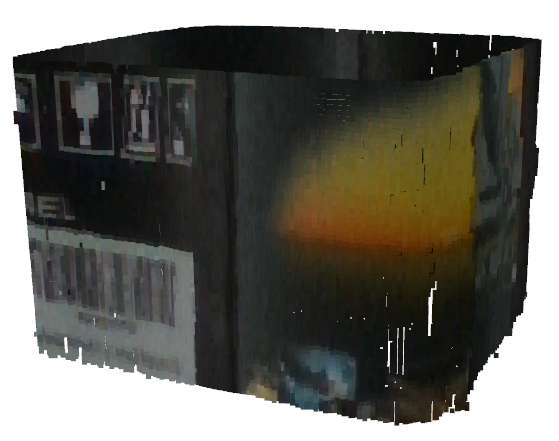
\includegraphics[scale=0.6]{pudelkoPointcloud.PNG}
    \end{minipage}
\quad
    \begin{minipage}[b]{0.45\linewidth}
        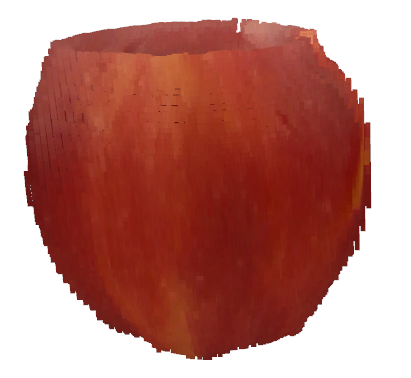
\includegraphics[scale=0.6]{jablkoPointcloud.PNG}

    \end{minipage}
\caption{Chmury punktów pudełka oraz jabłka.}
\label{fig:pointCloudFig}
\end{figure}

W celu sprawdzenia wpływu długości promienia kuli na ostateczny wygląd modelu dokonano porównania. Na rysunkach \ref{fig:appleComparison1},\ref{fig:appleComparison2},\ref{fig:boxComparison1} i \ref{fig:boxComparison2} znajdują się modele jabłka oraz pudełka na które został nałożony mesh korzystając z metody BPA. Dla każdego z nich sprawdzono wartość promienia R równą odpowiednio 2,5,7,10 razy średnia odległość pomiędzy punktami. Dla lepszego porównania zdjęcia modeli robiono pod podobnym kątem.


\begin{figure}[H]
\centering
    \begin{minipage}[b]{0.45\linewidth}
        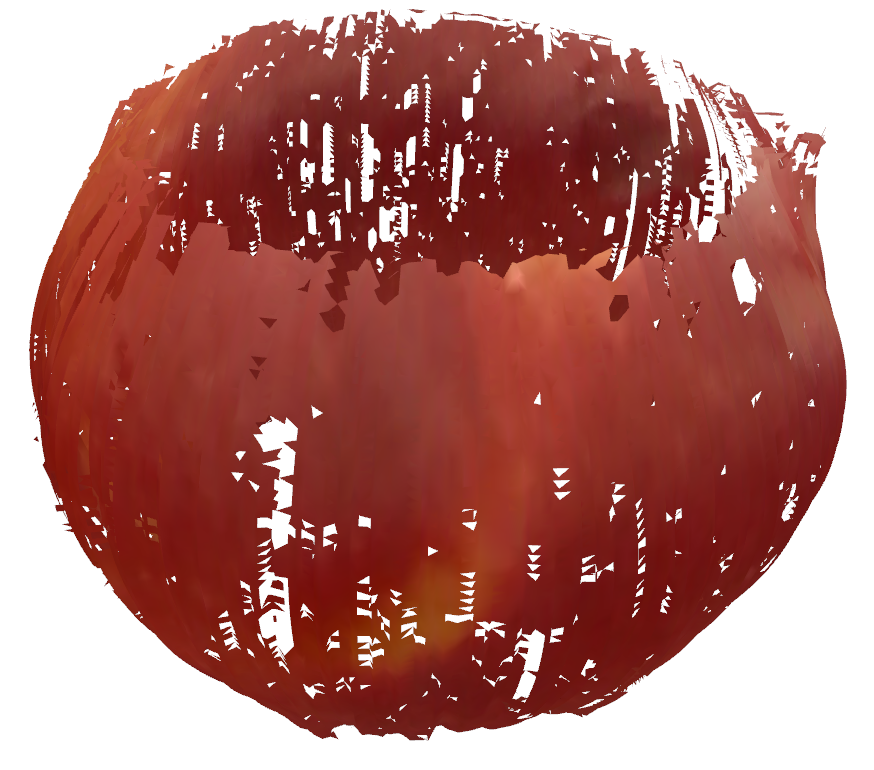
\includegraphics[scale=0.3]{bpaApple2x.PNG}
    \end{minipage}
\quad
    \begin{minipage}[b]{0.45\linewidth}
        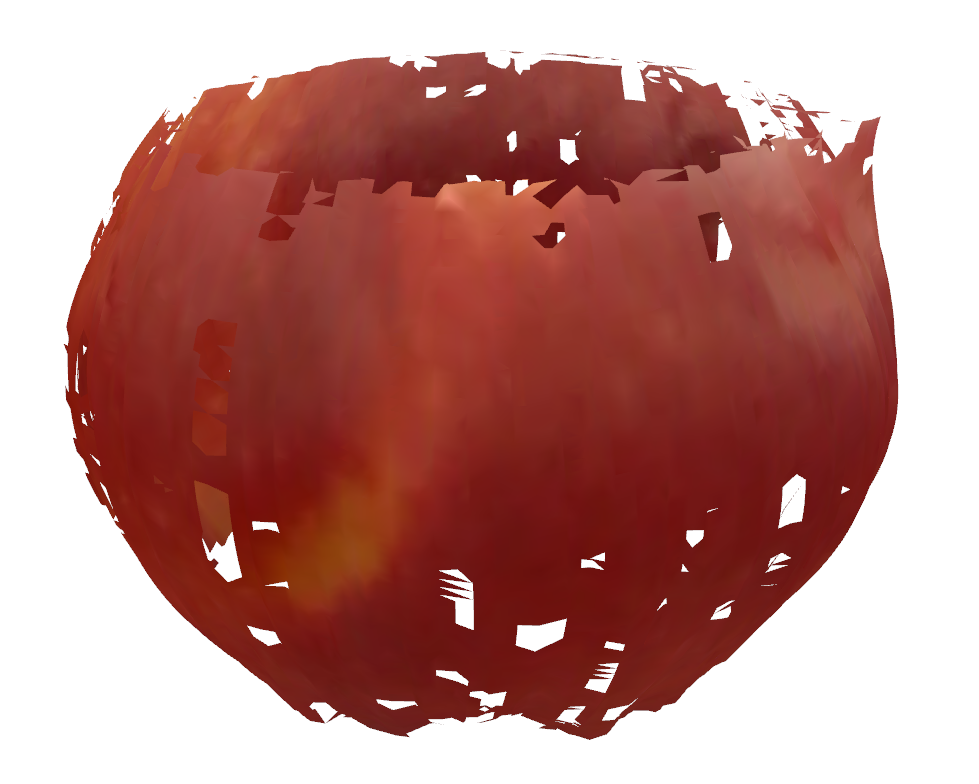
\includegraphics[scale=0.3]{bpaApple5x.PNG}
    \end{minipage}
\caption{Mesh BPA dla R=2$D_{mean}$ T=1.41 s oraz R=5$D_{mean}$ T=78 s .}
\label{fig:appleComparison1}
\end{figure}

\begin{figure}[H]
\centering
    \begin{minipage}[b]{0.45\linewidth}
        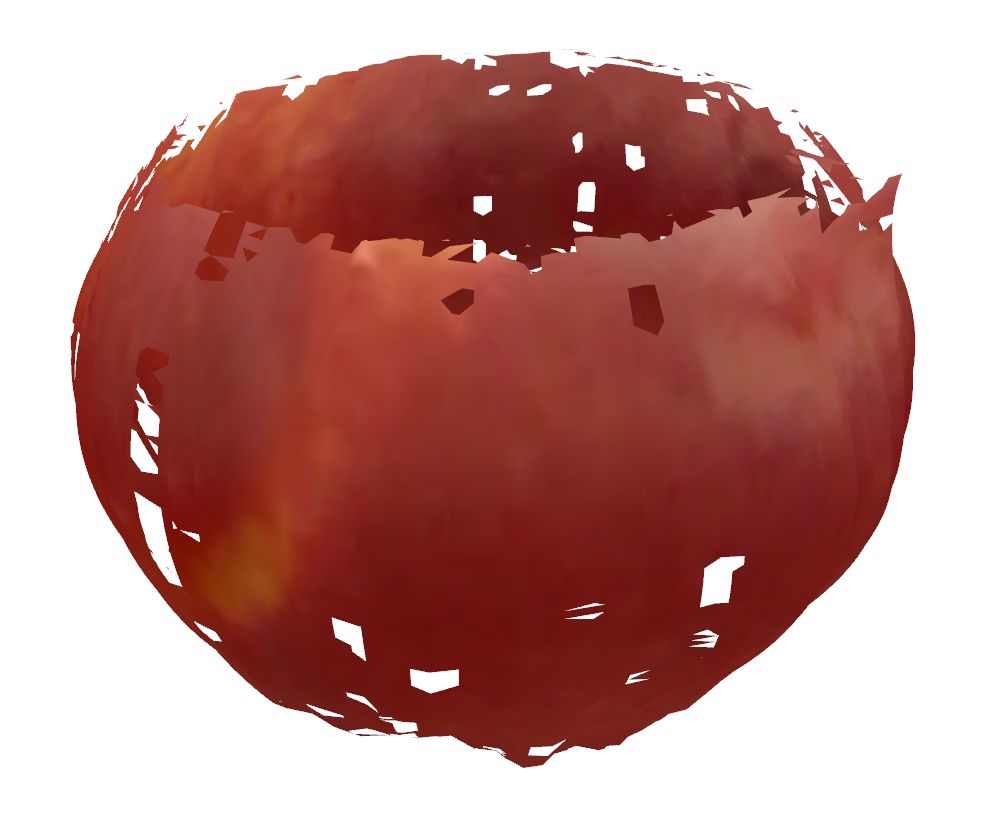
\includegraphics[scale=0.3]{bpaApple7x.PNG}
    \end{minipage}
\quad
    \begin{minipage}[b]{0.45\linewidth}
        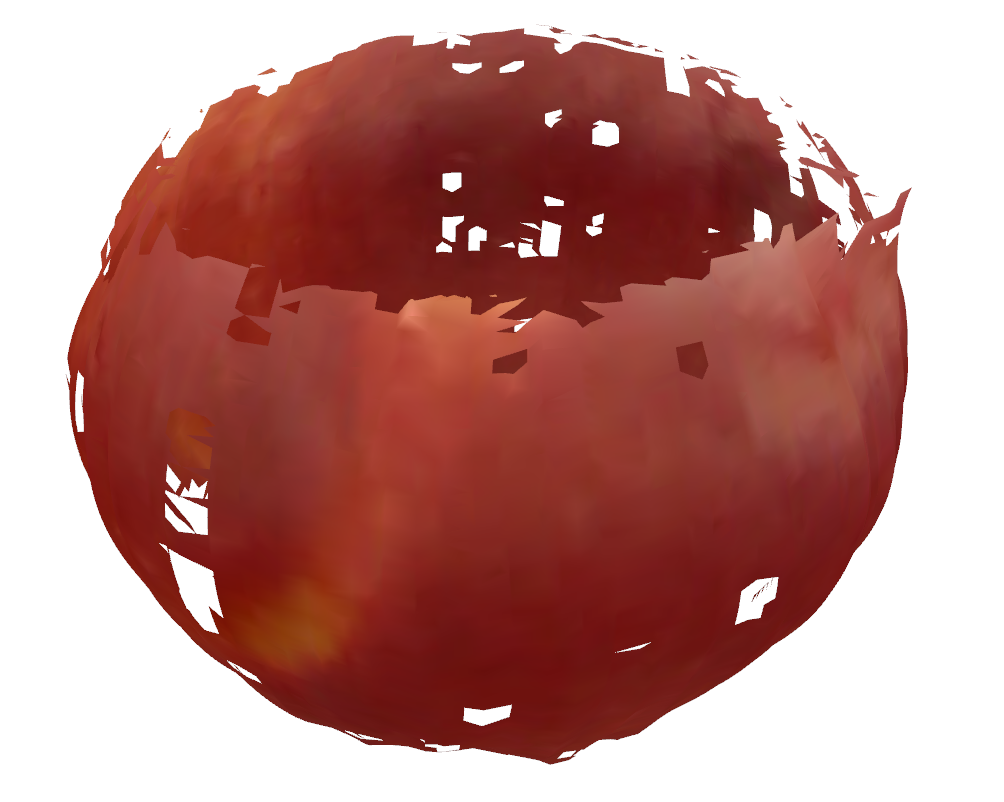
\includegraphics[scale=0.3]{bpaApple10x.PNG}
    \end{minipage}
\caption{Mesh BPA dla R=7$D_{mean}$ T=331 s oraz R=10$D_{mean}$ T=1532 s .}
\label{fig:appleComparison2}
\end{figure}

\begin{figure}[H]
\centering
    \begin{minipage}[b]{0.45\linewidth}
        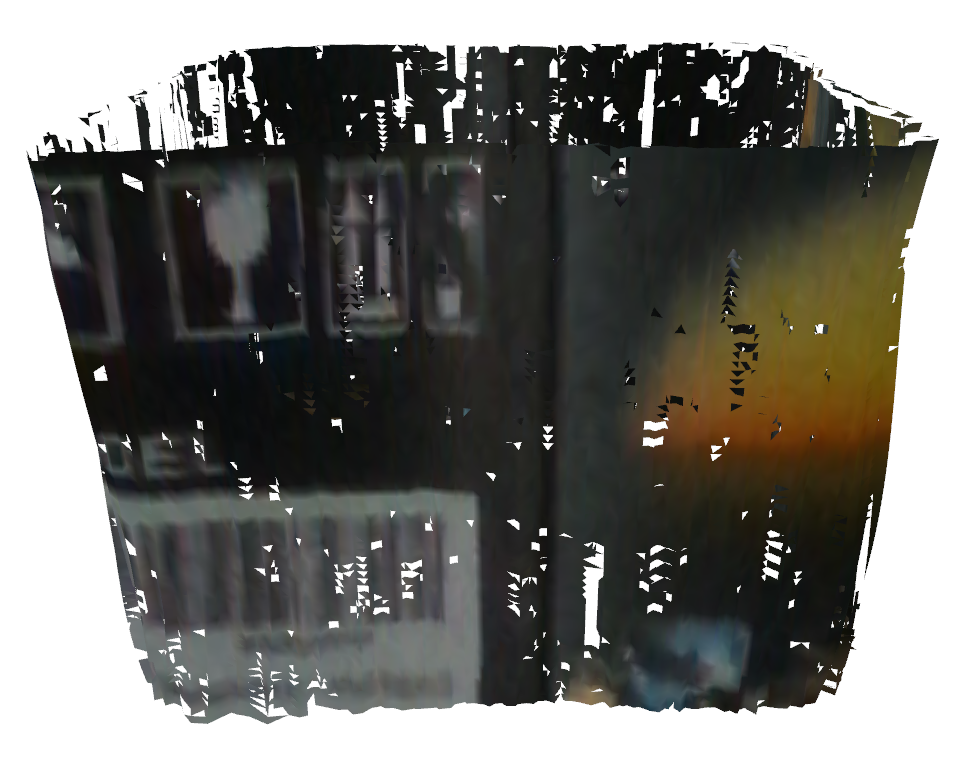
\includegraphics[scale=0.3]{bpaBox2x.PNG}
    \end{minipage}
\quad
    \begin{minipage}[b]{0.45\linewidth}
        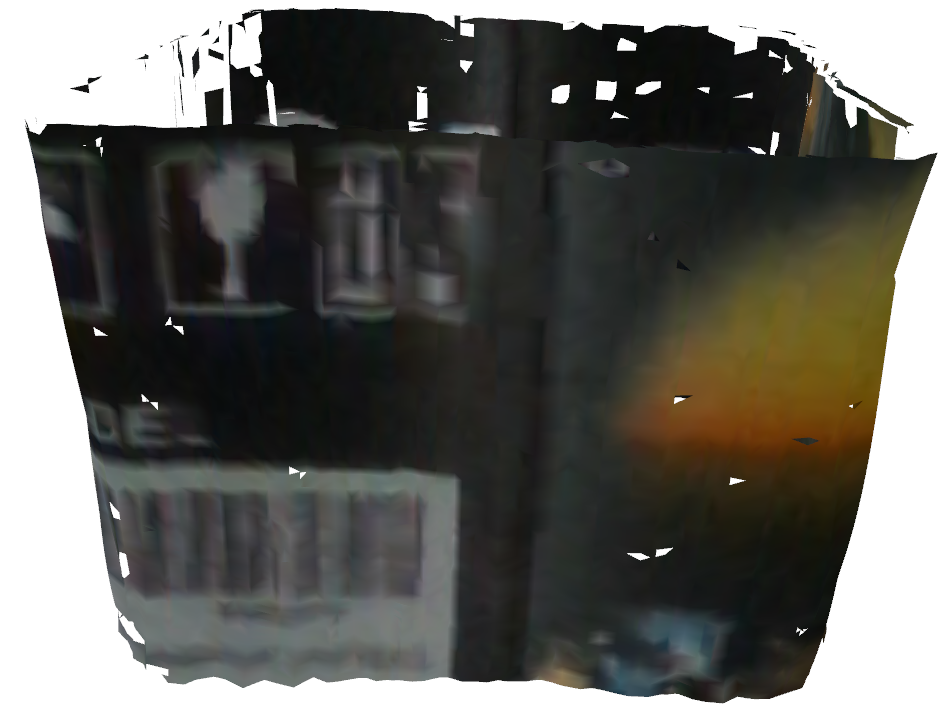
\includegraphics[scale=0.3]{bpaBox5x.PNG}
    \end{minipage}
\caption{Mesh BPA dla R=2$D_{mean}$ T=1.04 s oraz R=5$D_{mean}$ T=53 s .}
\label{fig:boxComparison1}
\end{figure}

\begin{figure}[H]
\centering
    \begin{minipage}[b]{0.45\linewidth}
        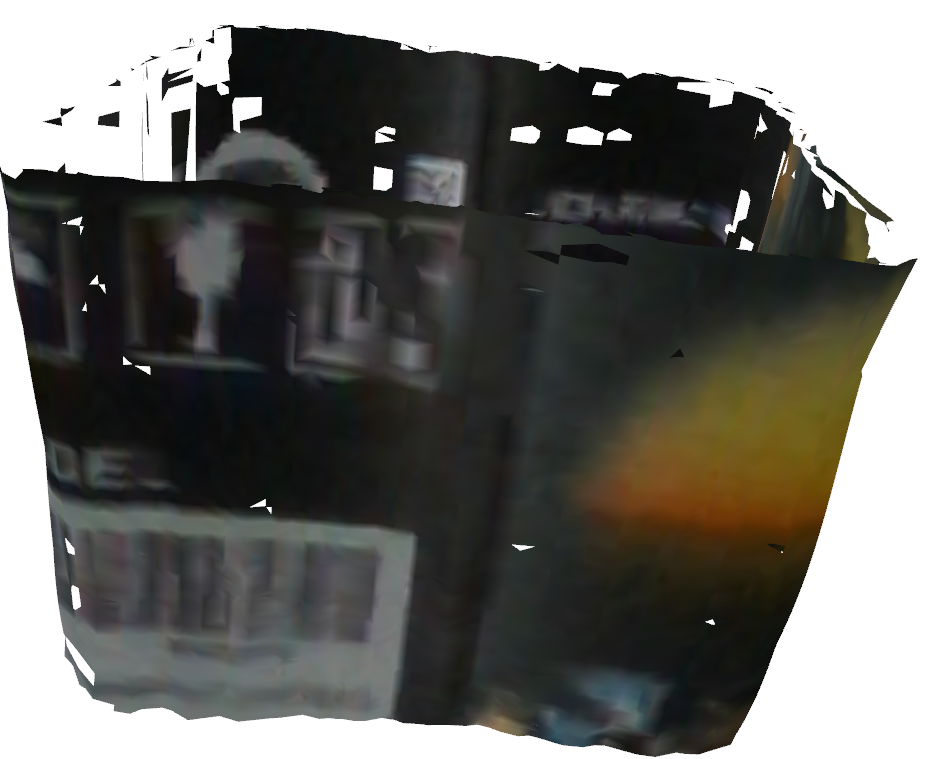
\includegraphics[scale=0.3]{bpaBox7x.PNG}
    \end{minipage}
\quad
    \begin{minipage}[b]{0.45\linewidth}
        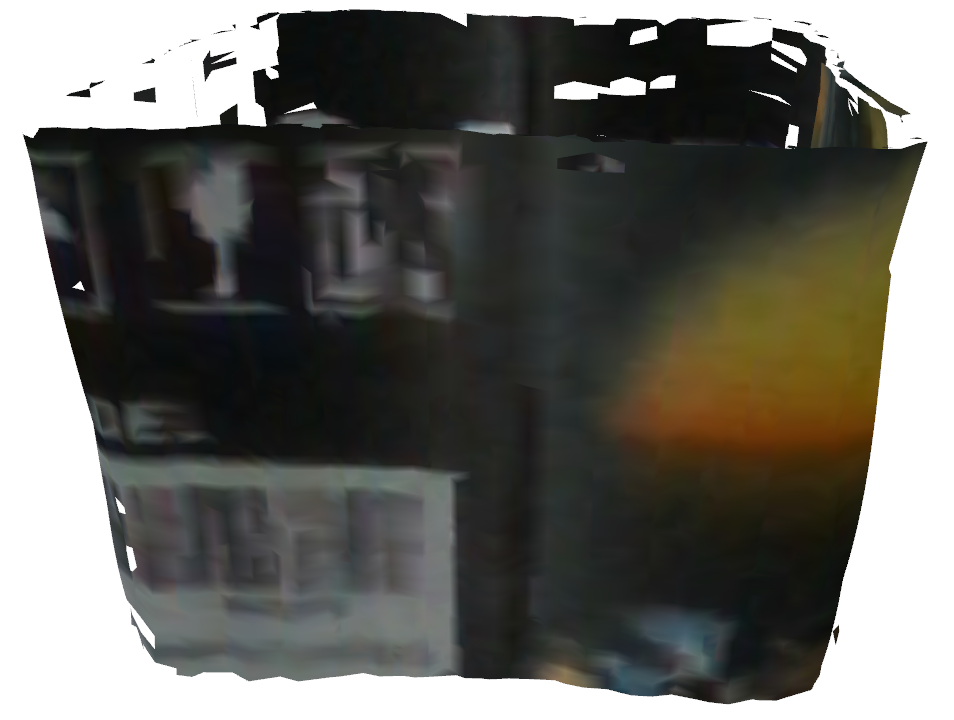
\includegraphics[scale=0.3]{bpaBox10x.PNG}
    \end{minipage}
\caption{Mesh BPA dla R=7$D_{mean}$ T=233 s oraz R=10$D_{mean}$ T=1071 s .}
\label{fig:boxComparison2}
\end{figure}
Na powyższym zestawieniu widać, że wygląd chmury punktów znacząco różni się od gotowego meshu. W modelu jest wiele luk, które należy zakryć. Dokonać tego można przez odpowiednie dobranie promienia kuli. Znaczący wpływ na luki ma nierównomierna gęstość rozłożenia punktów w chmurze. Dla długości promienia równej dwukrotnej średniej odległości punktów, na rysunku \ref{fig:appleComparison1} oraz \ref{fig:boxComparison1} widać znaczny ich odsetek. Zwiększenie promienia do 5 znacznie poprawia wypełnienie. Po tym etapie, dalsze powiększanie promienia wpływa nieznacznie na ostateczny wygląd.

Przy zwiększaniu promienia rośnie również czas obliczeniowy. Powodem tego jest większa ilość punktów w sąsiedztwie kuli. Dla każdego jej przesunięcia wymagane jest wyznaczenie sąsiadów z odległości 2R, co przy większym promieniu oznacza znaczną ilość punktów. Dla małej długości promienia czas obliczeń jest stosunkowo dobry. Algorytm zajmuje około 50 sekund. Można jednak zauważyć gwałtowną tendencję wzrostową. Zwiększenie o mniej niż 50 \% długości promienia, sprawia , że długość obliczeń wzrasta pięciokrotnie. W celu najlepszych wyników zarówno czasowych jak i wyglądu modeli należy empirycznie dobrać promień. Z obserwacji wynika, że promień równy trzykrotności średniej odległości punktów daje dobre rezultaty. Został to też potwierdzone w pracach naukowych \cite{mittleman1999ball}. Z ich badań wynika, że średnio w sąsiedztwie kierunku toczenia się kuli powinno znajdować się 20 punktów. Przy R=3$D_{mean}$ wzdłuż oraz wokół promienia znajduje się 17 punktów. Oznacza to, że empirycznie dobrany promień jest dobrym punktem startowym do poszukiwań.

\subsection{Algorytm Delaunay}
W autorskim programie została w całości zaimplementowana metoda triangulacji Delauny'a. W poniższej sekcji opisane zostaną wyniki pomiarów, wygenerowane modele oraz ich udoskonalenia w programie Blender. Na rysunku \ref{fig:delaBoxApple} ukazane zostały triangulacje Delaunay'a dla chmur punktów jabłka oraz pudełka.
\begin{figure}[H]
\centering
    \begin{minipage}[b]{0.45\linewidth}
        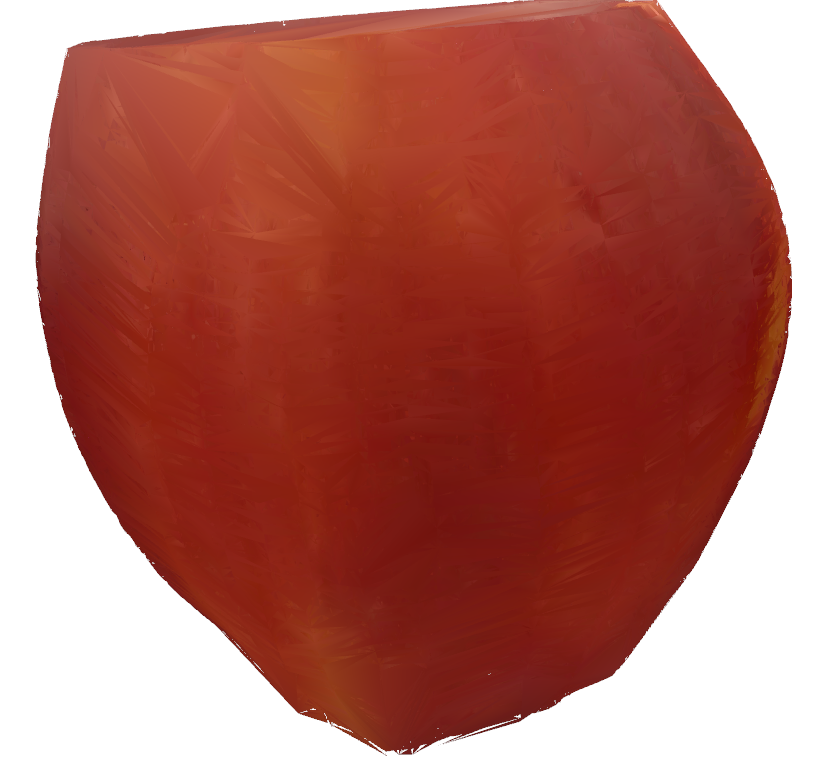
\includegraphics[scale=0.3]{jablkoDelNowe.PNG}
    \end{minipage}
\quad
    \begin{minipage}[b]{0.45\linewidth}
        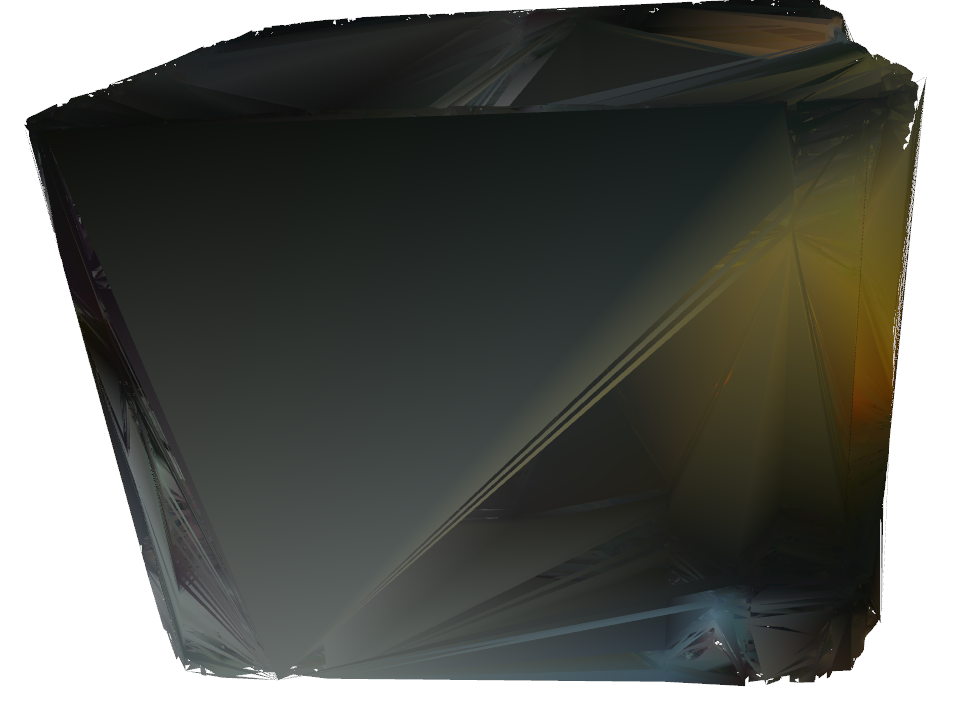
\includegraphics[scale=0.3]{delaunayBox.PNG}
    \end{minipage}
\caption{Mesh Delaunay dla jabłka oraz pudełka.}
\label{fig:delaBoxApple}
\end{figure}
Na rysunku powyżej można zauważyć najważniejszą różnicę algorytmu BPA od triangulacji Delauny'a. W przypadku pierwszego, wygenerowane modele zawsze zawierały pewien odsetek dziur. Jednakże, ze względu na istotę działania, modele uzyskane dzięki wykorzystaniu algorytmu Bowyera-Watsona ich nie zawierają. Wynika to z faktu, iż do poprawnego funkcjonowania tej metody, z każdej trójki punktów musi zostać utworzony trójkąt. Dzięki temu z każdego punktu w chmurze tworzona jest ściana ostrosłupa. Ponadto korzystając z danej metody, zostają również uzupełnione luki wynikające ze sposobu pomiaru. Akwizycja danych następuje z boku obiektu, dlatego nie istnieją dane o wierzchniej powierzchni modeli. Triangulacja Delaunay'a rozwiązuje ten problem, ponieważ graniczne punkty są łączone z pozostałymi na drugiej ścianie, tworząc w ten sposób dotychczas nieistniejącą ścianę. Kolory ścian wyznaczane są na podstawie wierzchołków trójkąta. 

Mankamentem tej metody jest fakt, że często ściany występujące w modelu są duże. Oznacza to, że niekiedy część krawędzi obiektu może zostać przysłonięta przez zbudowaną ścianę. Taka sytuacja została zaprezentowana na rysunku \ref{fig:delaBoxApple} w przypadku modelu pudełka. Kolory zostały wiernie oddane, jednak część z nich na siebie nachodzi, przysłaniając w ten sposób pozostałe. W przypadku jabłka ten problem nie występuje.

Wykorzystując program do obróbki modeli Blender, można dodatkowo wygładzić ściany z ostrych krawędzi powstałych w skutek triangulacji. Program zawiera szereg funkcji wpływających na wygląd gotowego meshy, zmieniając sposób w jaki światło się od nich odbija. Na rysunku \ref{fig:blenderDela} przedstawione zostały modele poddane obróbkom.

\begin{figure}[H]
\centering
    \begin{minipage}[b]{0.45\linewidth}
        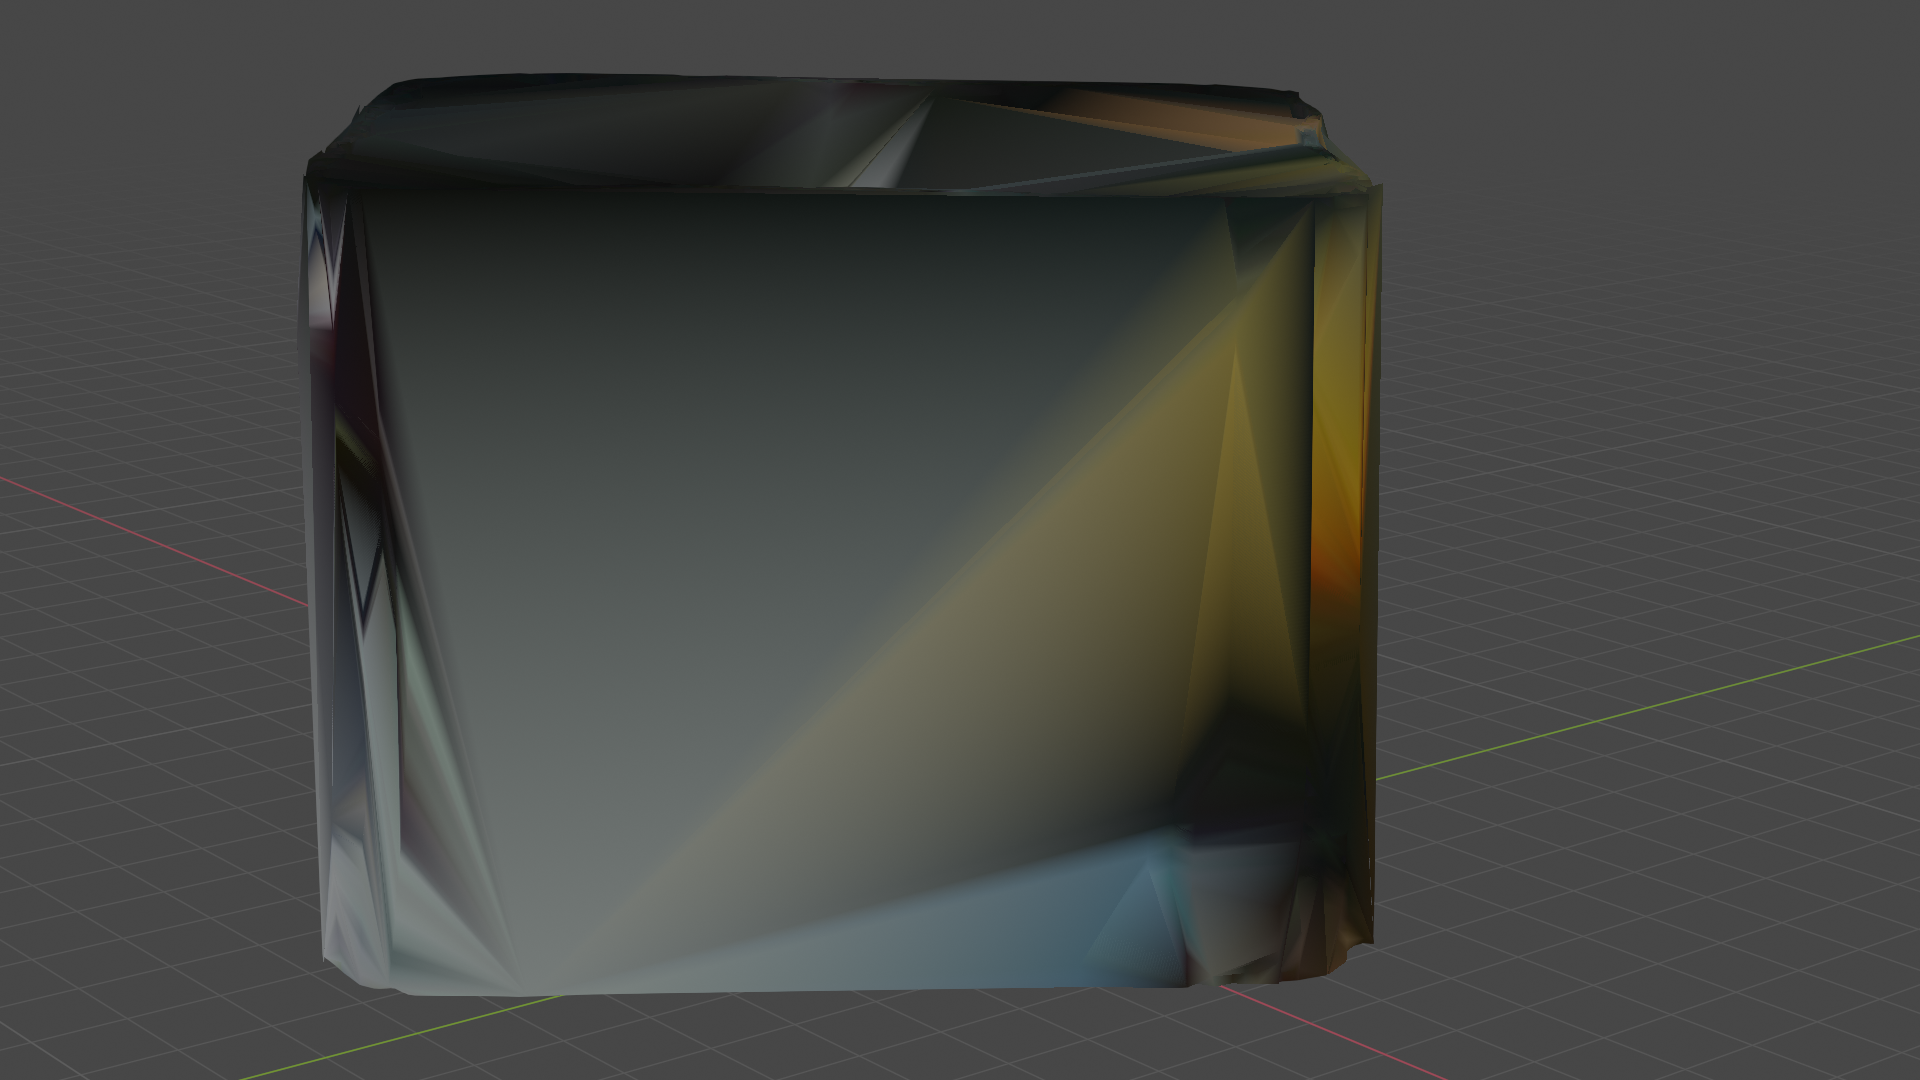
\includegraphics[scale=0.12]{delaBlendBoxgladkie.PNG}
    \end{minipage}
\quad
    \begin{minipage}[b]{0.45\linewidth}
        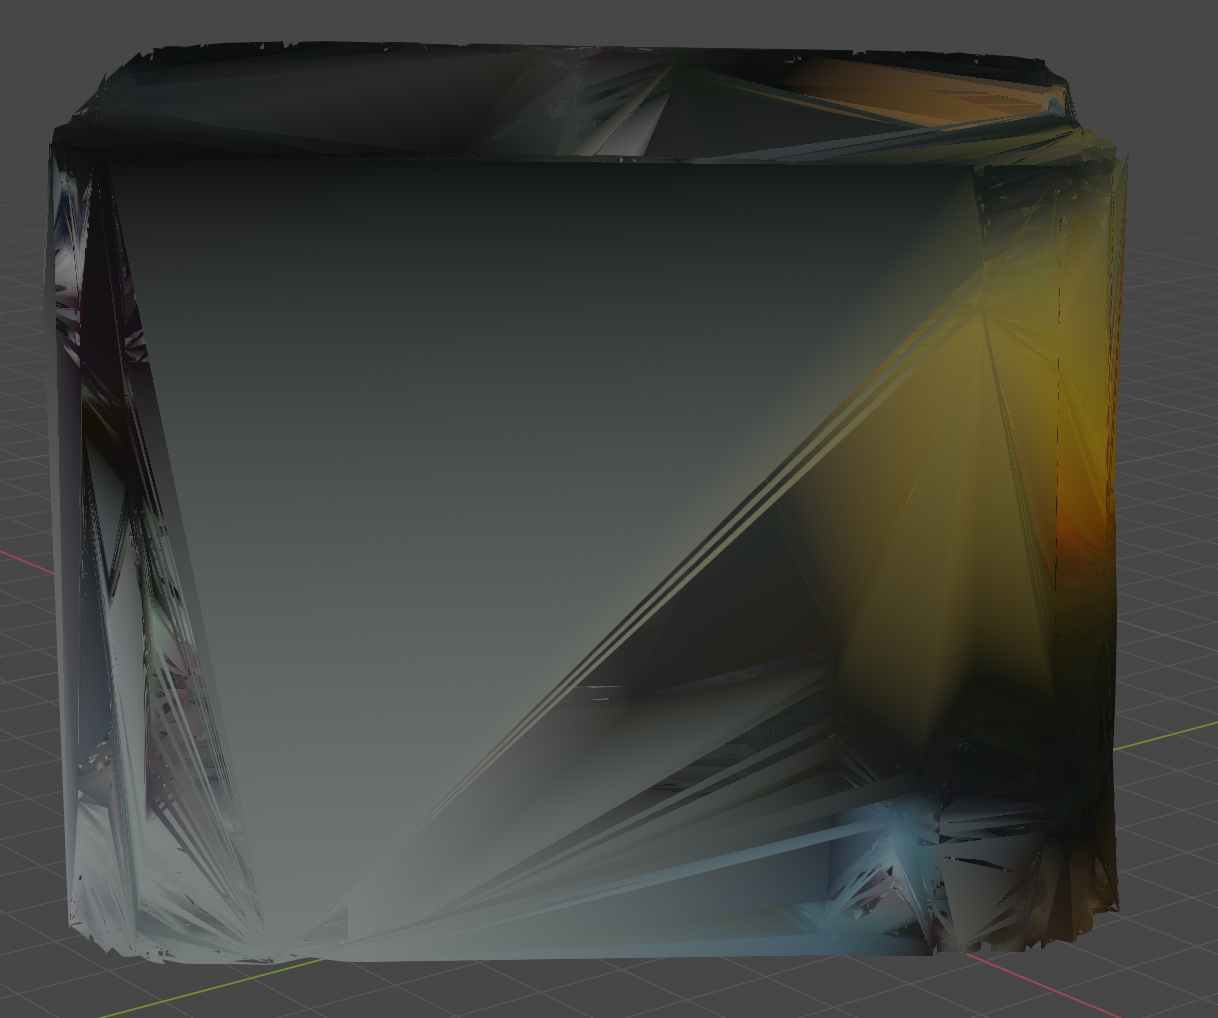
\includegraphics[scale=0.12]{delaBlendBoxNiegladkie.png}
    \end{minipage}
\caption{Mesh Delaunay dla pudełka przed i po wygładzaniu w programie Blender.}
\label{fig:blenderDela}
\end{figure}
Na powyższym rysunku przedstawiono modele przekształcone za pomocą programu Blender. Zastosowano funkcję flat do wyrównania poziomu cieni wokół wystających krawędzi, dzięki czemu stają się one mniej widoczne. Po lewej stronie wprowadzono funkcję, zakrywającą tylne krawędzie. Wykorzystując te metodę można uzyskać gładkie boki sześcianu, co wpływa pozytywnie na wygląd modelu. Część krawędzi przekształcono za pomocą edycji wierzchołków. Jest to funkcja pozwalająca na wygładzanie wystających wierzchołków trójkątów triangulacyjnych. Możliwe jest też podnoszenie tych, które leżą zbyt nisko, dzięki czemu ściany mają naturalny kształt. 
\begin{figure}[H]
  \centering
  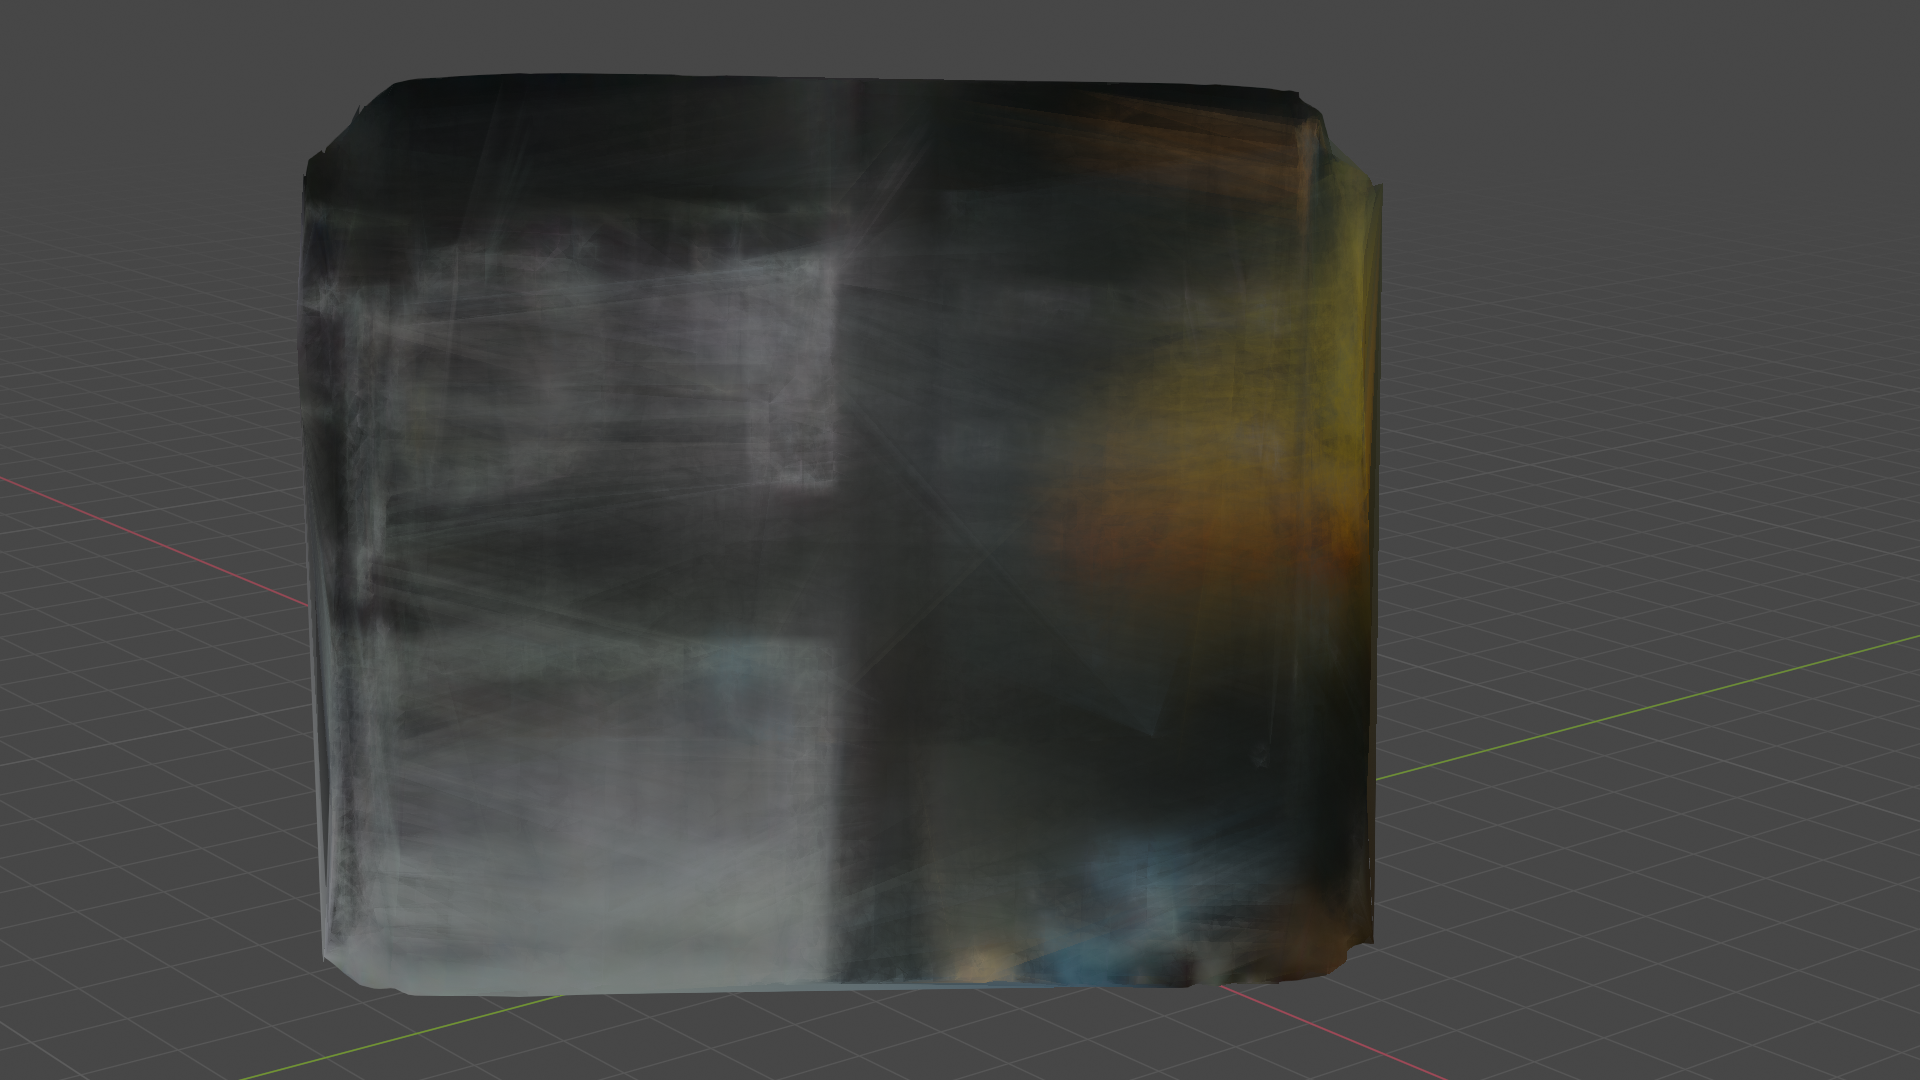
\includegraphics[scale=0.2]{delaBlendBoxXray.png}
  \caption{Ukryte ściany pudełka widoczne w programie Blender.}   
  \label{fig:pytcytpic}
\end{figure}
Na rysunku powyżej zastosowano funkcję Xray. Pozwala ona na wyświetlenie dolnych warstw obiektu. Wykorzystując to przekształcenie, można zauważyć, że triangulacja Delaunay'a działa poprawnie. Ściany które dotychczas były ukryte, ukazują faktyczną teksturę obiektu która pokrywa się z tą wygenerowaną przez chmurę punktów.

Ostatecznie wybrano triangulację Delaunay'a do przeprowadzania generacji meshu. Pomimo wad takich jak przykrywanie wierzchnich warstw powierzchni przez trójkąty daje ona dobre rezultaty. Ściany modelu nie zawierają dziur. Poprzez wykorzystanie tego algorytmu generowane zostają też ściany, które w przypadku BPA nie mogły zostać utworzone. Taka sytuacja jest dla dolnej oraz górnej ściany prostopadłościanu oraz jabłka. Delaunay generując trójkąty łączy również przeciwległe ściany zakrywając tym samym obszary nieobjęte przez chmurę punktów. Poprzez zastosowanie danej metody uzyskuje się zawsze taki sam rezultat. Wygląd modelu nie zależy od nastaw parametru, tak jak miało to miejsce w przypadku BPA. Usprawnia to proces konwersji fizycznych obiektów do postaci 3D,a dzięki programowi Blender można dodatkowo usunąć niepotrzebne trójkąty zakrywające pozostałe ściany.



